\section{Технический проект}
\subsection{Общая характеристика организации решения задачи}

Необходимо спроектировать и разработать компьютерную программу, позволяющую редактировать WAV аудиофайлы.

Компьютерная программа представляет собой комбинацию компьютерных инструкций и данных, позволяющую аппаратному обеспечению вычислительной системы выполнять вычисления или функции управления.

\subsection{Обоснование выбора технологии проектирования}

На сегодняшний день информационный рынок, поставляющий программные решения в выбранной сфере, предлагает множество продуктов, позволяющих достигнуть поставленной цели – разработки компьютерной программы для работы с аудио.

\subsubsection{Python}

Python — высокоуровневый язык программирования общего назначения с динамической строгой типизацией и автоматическим управлением памятью, ориентированный на повышение производительности разработчика, читаемости кода и его качества, а также на обеспечение переносимости написанных на нём программ.

\subsubsection{TKinter}

Tkinter --  кросс—платформенная событийно—ориентированная графическая Python—библиотека на основе средств Tk, написанная Стином Лумхольтом и Гвидо ван Россумом. Входит в стандартную библиотеку Python и предназначена для разработки графического интерфейса.

\subsubsection{NumPy}

NumPy -- открытая бесплатная Python—библиотека для работы с многомерными массивами, чаще всего используемая в анализе данных и обучении нейронных сетей.

\subsubsection{PySDL}

Python Simple DirectMedia Layer (PySDL) -- открытая бесплатная кроссплатформенная мультимедийная Python—библиотека, реализующая единый программный интерфейс к графической подсистеме, звуковым устройствам и средствам ввода для широкого спектра платформ. Данная библиотека активно используется при написании кроссплатформенных мультимедийных программ.

\subsubsection{Ctypes}

Ctypes -- Python—библиотека внешних функций, представляющая собой C--совместимые типы данных и позволяющая вызывать функции из DLL или разделяемых библиотек. Её можно использовать для оборачивания этих библиотек в чистый Python.

\subsection{Диаграмма компонентов}

Диаграмма компонентов описывает особенности физического представления разрабатываемой системы. Она позволяет определить архитектуру системы, установив зависимости между программными компонентами, в роли которых может выступать как исходный, так и исполняемый код. На рисунке \ref{diagram_comp:image} изображена диаграмма компонентов для проектируемой системы.

\begin{figure}[ht]
	\center{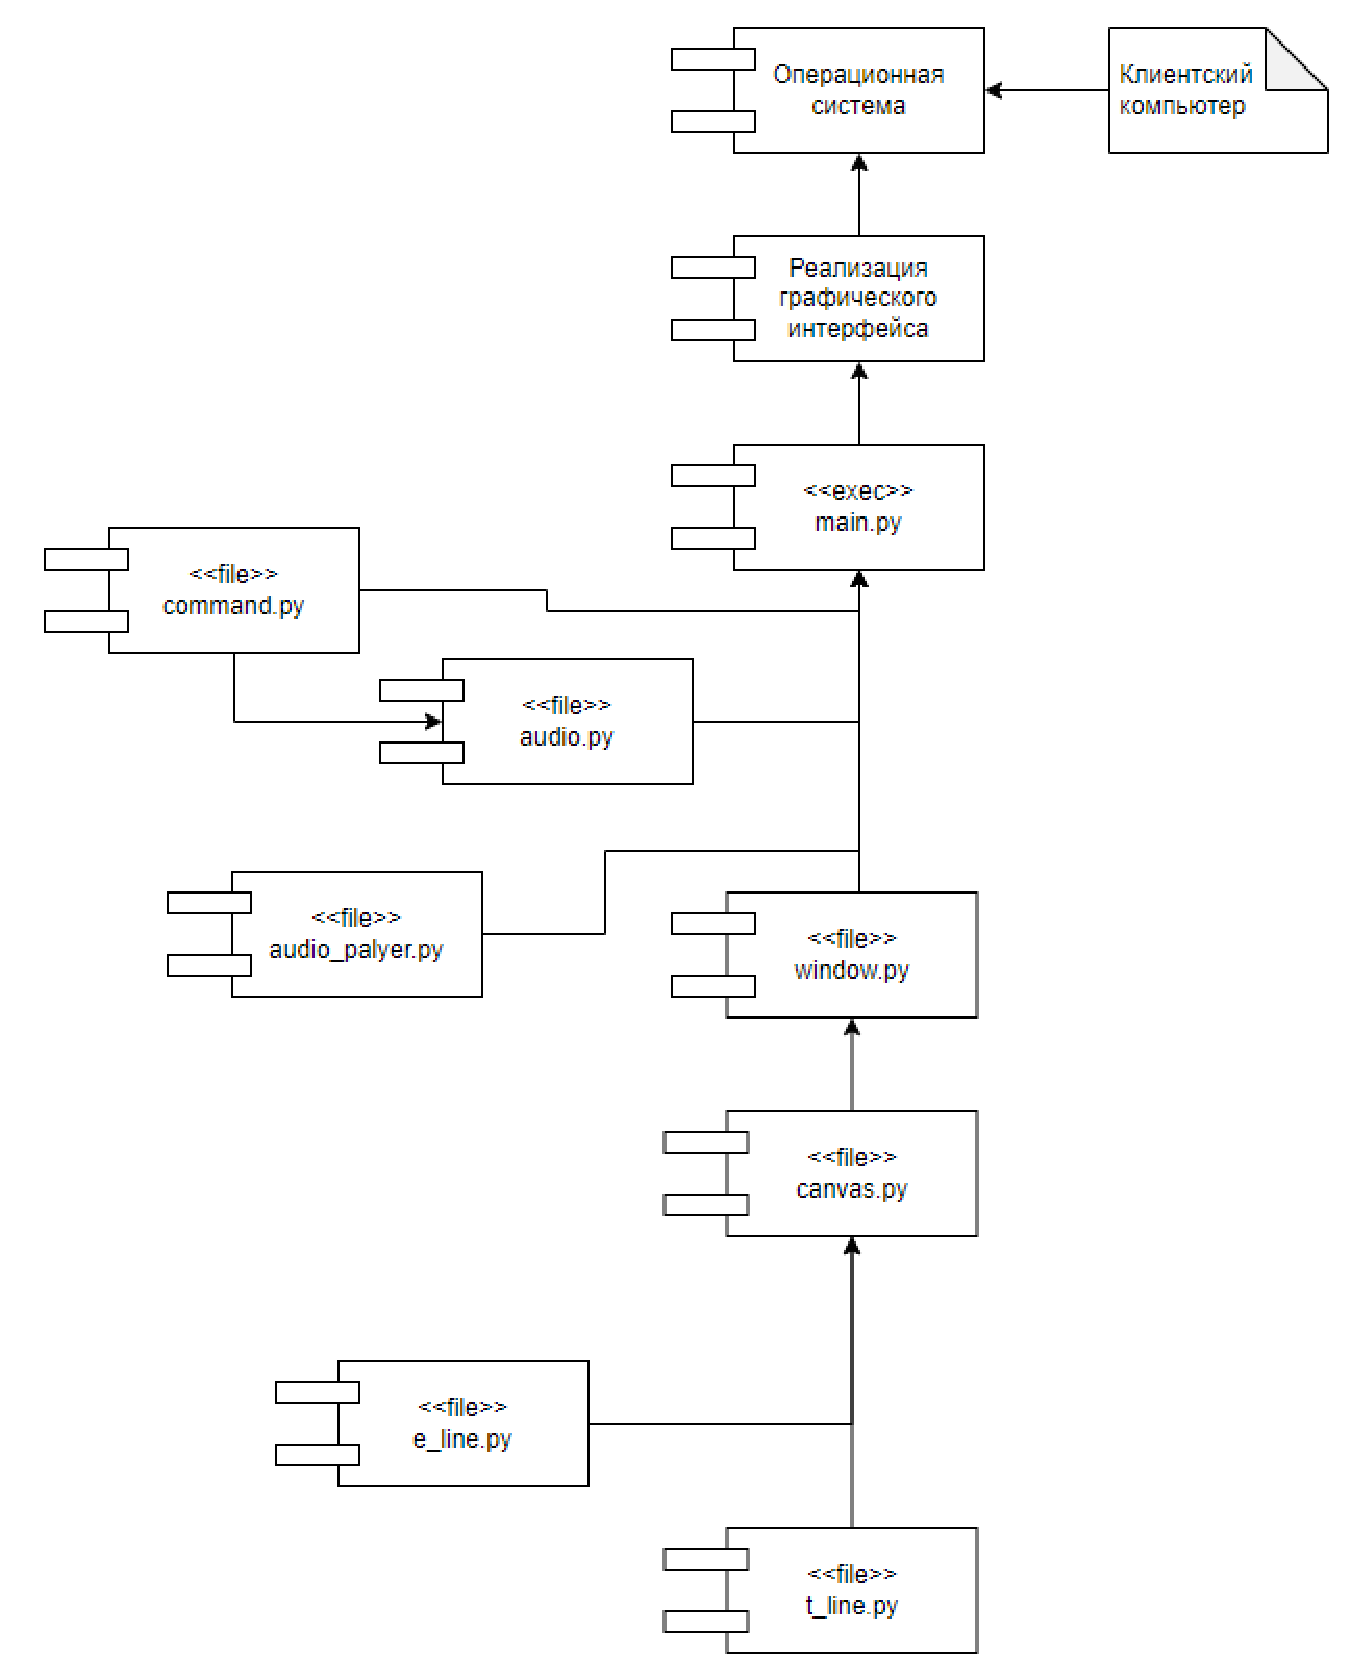
\includegraphics[width=0.7\linewidth]{diagram_comp}}
	\caption{Диаграмма компонентов}
	\label{diagram_comp:image}
\end{figure}

Основным исполняемым файлов является файл main.py, объединяющий в себе все другие компоненты. При запуске происходит создание графичексого интерфейса, посредством которого пользователь может взаимодействовать с программой. 

\subsection{Содержание информационных блоков. Основные сущности}

Проанализировав требования, можно выделить 5 основных сущностей:
\begin{itemize}
	\item "<Аудио">;
	\item "<Аудиоплеер">;
	\item "<Окно">;
	\item "<Холст">;
	\item "<Команда">.
\end{itemize}

Ниже представлены таблицы составов перечисленных выше сущностей.

\begin{xltabular}{\textwidth}{|p{2.1cm}|p{2cm}|l|X|}
	\caption{Атрибуты сущности "<Аудио">}\\ \hline
	\label{news:table}
	\thead{Поле} & \thead{Тип} & \thead{Начальное значение} & \thead{Описание} \\ \hline
	\thead 1 & \thead 2 & \thead 3 & \thead 4 \\ \hline
	\endfirsthead
	\continuecaption{Продолжение таблицы \ref{news:table}}
	\thead 1 & \thead 2 & \thead 3 & \thead 4 \\ \hline
	\finishhead
	nchannels & Integer & 0 & Количество каналов \\ \hline 
	sampwidth & Integer & 0 & Размер сэмплов \\ \hline 
	framerate & Integer & 0 & Частота сэмплов \\ \hline 
	nframes & Integer & 0 & Количество сэмплов \\ \hline 
	comptype & String & NONE & Тип сжатия \\ \hline 
	compname & String & not compressed & Название сжатия \\ \hline 
	chunksize & Integer & 0 & Размер буфера за ед. времени \\ \hline 
	copy buffer & Numpy. array & Numpy.array([], dtype=int16) & Буфер для хранения скопированной области \\ \hline 
	signals data & Numpy. array & Numpy.array([], dtype=int16) & Буфер для хранения прочитанных сэмплов \\ \hline 
	duration & Float & 0.0 & Длительность
\end{xltabular}

\begin{xltabular}{\textwidth}{|p{2cm}|p{2cm}|l|X|}
	\caption{Атрибуты сущности "<Аудиоплеер">}\\ \hline
	\label{news2:table}
	\thead{Поле} & \thead{Тип} & \thead{Начальное значение} & \thead{Описание} \\ \hline
	\thead 1 & \thead 2 & \thead 3 & \thead 4 \\ \hline
	\endfirsthead
	\continuecaption{Продолжение таблицы \ref{news2:table}}
	\thead 1 & \thead 2 & \thead 3 & \thead 4 \\ \hline
	\finishhead
	audio & Audio & Audio(kwargs) & Объект класса Audio \\ \hline 
	bactive & Bool & False & Флаг для проверки активности \\ \hline 
	bplaying & Bool & False & Флаг для проверки проигрывания \\ \hline 
	chunk & Bytes & Пустрокая строка байтов & Проигрываемый аудиобуфер \\ \hline 
	volume & Integer & 100 & Громкость \\ \hline 
	start & Float & 0.0 & Время начала выбранной области \\ \hline 
	start index & Integer & 0 & Индекс начала выбранной области в буфере \\ \hline 
	end & Float & 0.0 & Время конца выбранной области \\ \hline 
	end index & Integer & 0 & Индекс конца выбранной области в буфере \\ \hline 
	current & Float & 0.0 & Время проигрывания
\end{xltabular}

\begin{xltabular}{\textwidth}{|p{2cm}|p{2cm}|l|X|}
	\caption{Атрибуты сущности "<Окно">}\\ \hline
	\label{news3:table}
	\thead{Поле} & \thead{Тип} & \thead{Начальное значение} & \thead{Описание} \\ \hline
	\thead 1 & \thead 2 & \thead 3 & \thead 4 \\ \hline
	\endfirsthead
	\continuecaption{Продолжение таблицы \ref{news3:table}}
	\thead 1 & \thead 2 & \thead 3 & \thead 4 \\ \hline
	\finishhead
	scrollbar & Scrollbar & Scrollbar (kwargs) & Ползунок для просмотра дорожки \\ \hline 
	canvas & Canvas & Canvas(kwargs) & Вспомагательный холст \\ \hline 
	scrollable frame & Frame & Frame(kwargs) & Вспомагательная прокручиваемая рамка \\ \hline 
	scrollable canvas & Scrollable Canvas() & Scrollable Canvas(kwargs) & Прокручиваемый холст \\ \hline 
	frame & Frame & Frame(kwargs) & Главная рамка
\end{xltabular}

\begin{xltabular}{\textwidth}{|p{2cm}|p{2cm}|l|X|}
	\caption{Атрибуты сущности "<Холст">}\\ \hline
	\label{news4:table}
	\thead{Поле} & \thead{Тип} & \thead{Начальное значение} & \thead{Описание} \\ \hline
	\thead 1 & \thead 2 & \thead 3 & \thead 4 \\ \hline
	\endfirsthead
	\continuecaption{Продолжение таблицы \ref{news4:table}}
	\thead 1 & \thead 2 & \thead 3 & \thead 4 \\ \hline
	\finishhead
	loaded & Bool & False & Флаг для проверки загрузки холста \\ \hline 
	player & AudioPla- yer & AudioPlayer(kwargs) & Объект класса AudioPlayer \\ \hline 
	signals & List & [] & Группированные значения амплитуд \\ \hline 
	signals count & Integer & 1 & Количество линий холста \\ \hline 
	pixels per second & Integer & 12 & Количество пикселей, необходимое для отображения 1 секунды звука \\ \hline 
	bdrawing & Bool & False & Флаг для проверки отрисовки \\ \hline 
	block & Bool & False & Флаг для блокировки границ \\ \hline 
	s line & EdgeLine & EdgeLine(kwargs) & Граница начала области \\ \hline 
	e line & EdgeLine & EdgeLine(kwargs) & Граница конца области \\ \hline 
	t line & TimeLine & TimeLine(kwargs) & Линия времени \\ \hline 
	labels & List & [0, [Label()]] & Временные отметки
\end{xltabular}

\begin{xltabular}{\textwidth}{|p{2cm}|p{2cm}|l|X|}
	\caption{Атрибуты сущности "<Команда">}\\ \hline
	\label{news5:table}
	\thead{Поле} & \thead{Тип} & \thead{Начальное значение} & \thead{Описание} \\ \hline
	\thead 1 & \thead 2 & \thead 3 & \thead 4 \\ \hline
	\endfirsthead
	\continuecaption{Продолжение таблицы \ref{news5:table}}
	\thead 1 & \thead 2 & \thead 3 & \thead 4 \\ \hline
	\finishhead
	audio & Audio() & Audio(kwargs) & Объект класса Audio \\ \hline 
	start index & Integer & Задается при вызове конструктора & Индекс начала выбранной области в буфере \\ \hline 
	end index & Integer & Задается при вызове конструктора & Индекс конца выбранной области в буфере \\ \hline 
	buffer & Numpy. array() & [] & Неизмененный фрагмент аудио
\end{xltabular}

В системе предусмотрен внутренний механизм связи между разделами и элементами информационных блоков, поэтому введения дополнительных идентификаторов при реализации связей между сущностями не предполагается.

Экземпляры сущностей реализуются в информационных блоках посредством элементов, атрибуты сущности – посредством полей и свойств элемента. 
